% Gemini theme
% https://github.com/anishathalye/gemini

\documentclass[final]{beamer}

% ====================
% Packages
% ====================

\usepackage[T1]{fontenc}
\usepackage{lmodern}
\usepackage[orientation=landscape size=a0,scale=1.0]{beamerposter}
\usetheme{gemini}
\usecolortheme{gemini}
\usepackage{graphicx}
\usepackage{booktabs}
\usepackage{tikz}
\usepackage{pgfplots}
\usepackage{ragged2e}
\pgfplotsset{compat=1.14}

% ====================
% Lengths
% ====================

% If you have N columns, choose \sepwidth and \colwidth such that
% (N+1)*\sepwidth + N*\colwidth = \paperwidth
\newlength{\sepwidth}
\newlength{\colwidth}
\setlength{\sepwidth}{0.025\paperwidth}
\setlength{\colwidth}{0.3\paperwidth}

\newcommand{\separatorcolumn}{\begin{column}{\sepwidth}\end{column}}

% ====================
% Title
% ====================

\title{Generative Adversarial Active Learning for
	Unsupervised Outlier Detection}

\author{Yezheng Liu \inst{1} \and Zhe Li \inst{2} \and  Chong Zhou \inst{2} Yuanchun Jiang \inst{2} \and Jianshan Sun \inst{2}  \and Meng Wang \inst{2} \and Xiangnan He \inst{2} }

\institute[shortinst]{\inst{1} Some Institute \samelineand \inst{2} Another Institute}

% ====================
% Footer (optional)
% ====================

\footercontent{
  \href{https://github.com/NING0121/poster_latex}{https://github.com/NING0121/poster\_latex} \hfill
  Methods and Applications for Anomaly Detection 2022, ChengDu, SiChuan --- 147 and 080 \hfill
  \href{1104120243@qq.com}{1104120243@qq.com}
}
% (can be left out to remove footer)

% ====================
% Logo (optional)
% ====================

% use this to include logos on the left and/or right side of the header:
% \logoright{\includegraphics[height=7cm]{logo1.pdf}}
% \logoleft{\includegraphics[height=7cm]{logo2.pdf}}

% ====================
% Body
% ====================

\begin{document}

\begin{frame}[t]
\begin{columns}[t]
\separatorcolumn

\begin{column}{\colwidth}

  \begin{block}{INTRODUCTION}

    \textbf{OUTLIERS} refer to the observations that have significantly different characteristics from the other data. Due to the critical and interesting insights they often provide, outlier detection technologies play important roles in various application domains. Such as the abnormal trajectory and moving object detection, fraud detection, emerging topic detection and medical information detection.

  \end{block}


  \begin{block}{RELATED WORK}

    Here we briefly summarize some of the previous work on outlier detection, including the following three main approaches.

    \begin{itemize}
    	
      \item \textbf{Classic Outlier Detection Methods:} \justifying Gaussian mixture model (GMM), kth nearest neighbor (kNN), local reachability density (LOF), fast angle-based outlier detection (FastABOD) and so on.
      \item \textbf{AGPO-Based Outlier Detection Methods:} \justifying One-Class Random Forests (OCRF), Active-Outlier method (AO) and so on.
      \item \textbf{GAN-Based Outlier Detection Methods:}
      \justifying convolutional generative adversarial network (AnoGAN) and our methods.
      
    \end{itemize}

  \end{block}

  \begin{alertblock}{METHODOLOGY}
	
	\textbf{Core idea}: view the outlier detection as a binary classification problem
	
	Given a data set, each data will have a label indicating normal/abnormal (normal=1, abnormal=0). Anomaly detection is about finding a boundary that separates the abnormal data from the normal data. The optimal bound can be obtained by minimizing this objective function as follows. The optimal boundary can be determined by minimizing the loss function $L_{\zeta}$ of $\zeta(x)$.
	
	$$
	L_{\zeta}= -\sum_{i=1}^{n}(c_ny_i\log(\zeta(x_i))+c_o(1-y_i)\log(1-\zeta(x_i)))
	$$
	
	where $C_0$ and $C_n$ are the misclassification costs of outlier. $\zeta(x)\in(0,1)$ is a scoring function.
	
	Therefore, we can assume that the density around the abnormal data is lower than the density of the normal data. This is shown in the figure below.
	
	\begin{figure}
		\centering
		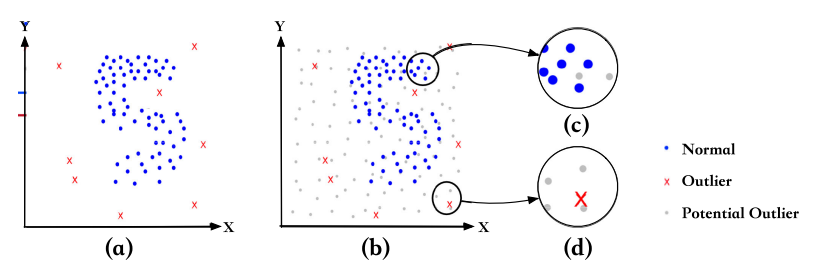
\includegraphics[scale=1]{figures/figure 1.png}
		\caption{Illustration of the AGPO-based outlier detection mechanism.}
		%Normal examples are shown with blue dots, outliers with red “x”, and generated potential outliers with gray dots.
	\end{figure}

	\begin{equation}\nonumber
		\begin{aligned}
			\zeta(x|\rho(x)\geq\tau)\rightarrow1,\\
			\zeta(x|\rho(x)\leq\tau)\rightarrow0,
		\end{aligned}
	\end{equation}
    \begin{figure}
	    \centering
	    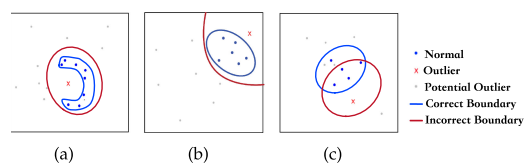
\includegraphics[scale=1.5]{figures/figure 2.png}
	    \caption{Illustration of the detection performance of the classifier $C(x)$ in three cross-sectional data drilled from high-dimensional datasets. The correct boundaries are shown with blue lines and incorrect boundaries with red lines. }
    \end{figure}
	$$
	L_C= -\frac{1}{2n}\sum_{i=1}^{2n}(y_i\log(C(x_i))+(1-y_i)\log(1-C(x_i)))
	$$
  \end{alertblock}

\end{column}

\separatorcolumn

\begin{column}{\colwidth}

  \begin{exampleblock}{Generative Adversarial Active Learning for Outlier Detection}
  	
  
   
  	\heading{Single-Objective Generative Adversarial
  		Active Learning}
  	$$
  	\min_{\theta_g}\max_{\theta_d}V(D,G)=\mathbb{E}_{x~p_{data}}[\log D(x)]+\mathbb{E}_{z~p_{z}}[\log(1-D(x))]
  	$$
  	
  	\begin{figure}
  		\centering
  		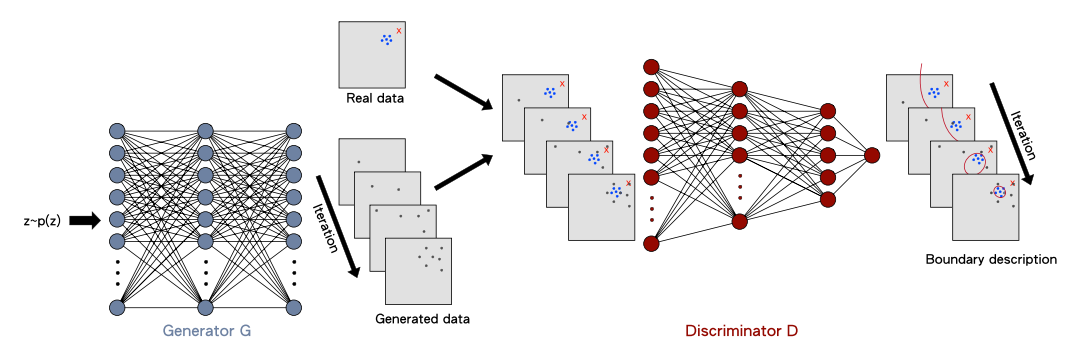
\includegraphics{figures/SO-GAAL.png}
  		\caption{The detection process of SO-GAAL based outlier detection algorithm.}
  		% At the beginning of training, generator $G$ cannot generate a sufficient number of potential outliers around the real data, which causes the discriminator $D$ to describe a rough boundary. But, after several iterations, the generator $G$ gradually learns the generation mechanism of real data based on the mini-max game between $G$ and $D$, and generates an increasing number of informative potential outliers. As a result, the discriminator $D$ can describe a correct boundary around the concentrated data points.
  	\end{figure}
  
    \begin{figure}
  	   \centering
  	   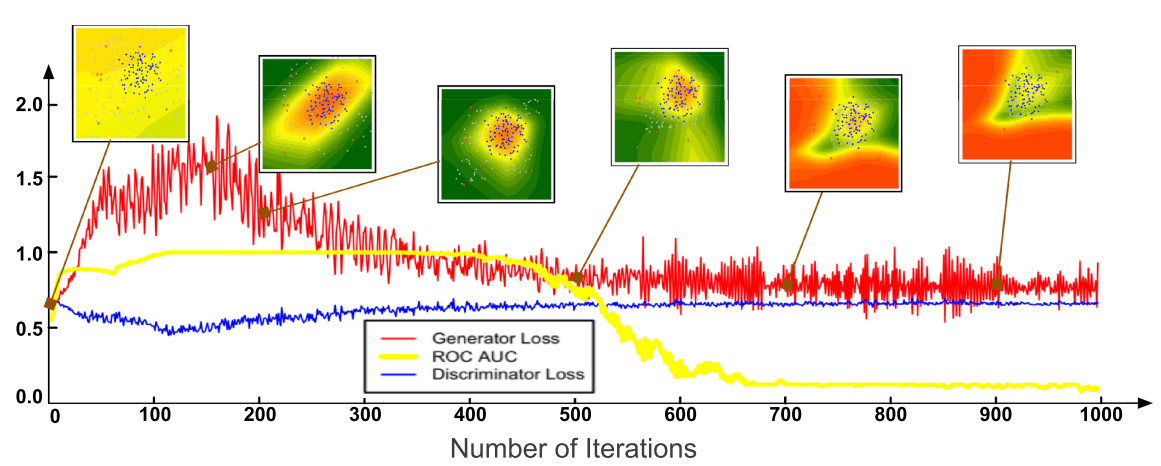
\includegraphics[scale=0.9]{figures/process of SO-GAAL.png}
  	   \caption{The optimization process of SO-GAAL based outlier detection.}
  	   % The generator loss is shown with the red line, discriminator loss with the blue line, and AUC with the yellow line. Gradient color in the top six pictures indicates the probability that the point is an outlier, and data points closer to the green area are more likely to be outliers. Due to all potential outliers occur inside or close to part of the real data, the accuracy of SO-GAAL drops dramatically when the mini-max game reaches the Nash equilibrium 
    \end{figure}
  	
  	\heading{Multiple-Objective Generative Adversarial Active Learning}
  	
    $$
    \max_{\theta_d}V_D=\frac{1}{2n}[\sum_{j=1}^{n}\log(D(x^{(j)})) + \sum_{i=1}^{k}\sum_{j=1}^{n_i}\log(1-D(G_i(z_i^{(j)})))]
    $$
    
    $$
    \min_{\theta_{g_i}}V_{G_i}=-\frac{1}{n}\sum_{j=1}^{n}[T_i\log(D(G_i(x^{(j)}))) + (1-T_i)\log(1-D(G_i(z_i^{(j)})))]
    $$
    
    \begin{figure}
    	\centering
    	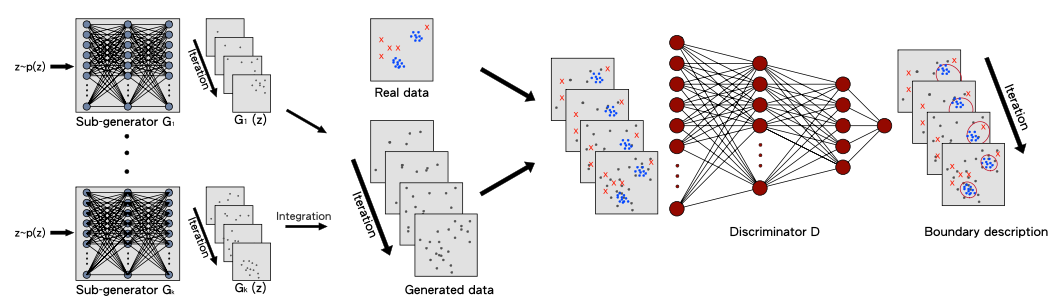
\includegraphics{figures/MO-GAAL.png}
    	\caption{The detection process of MO-GAAL based outlier detection algorithm.}
    	% MO-GAAL consists of $k$ sub-generators $G_{1:k}$, which generate different reference distributions for different data subsets. Although there are two clusters in the dataset, integrated potential outliers still provide a reasonable reference distribution to assist the discriminator $D$ in describing a correct boundary around the concentrated data points. 
    \end{figure}

    \begin{figure}
        \centering
	    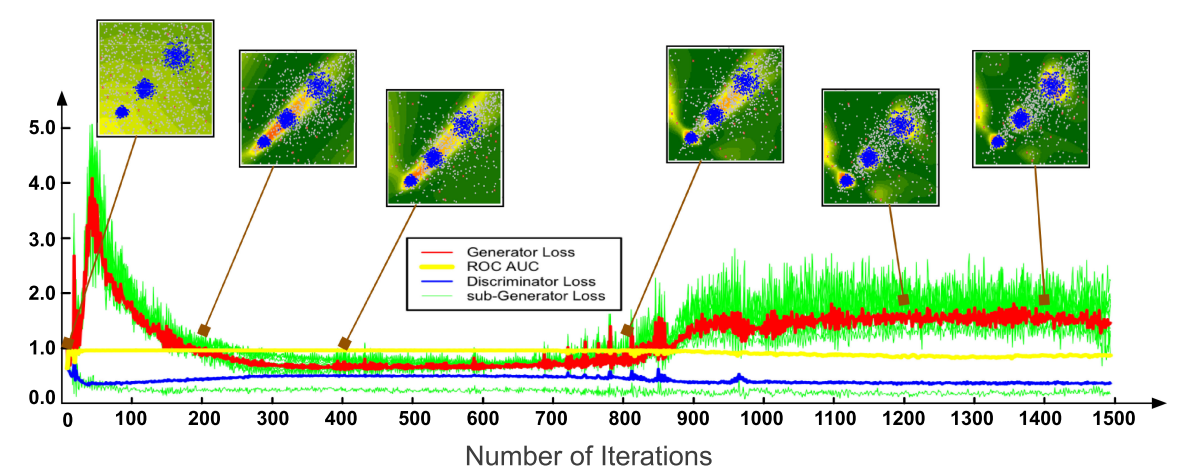
\includegraphics[scale=0.9]{figures/process of MO-GAAL.png}
	    \caption{The optimization process of MO-GAAL based outlier detection.}
	    % The meaning of the color is the same as the Fig. 4, and the sub-generator loss is shown with a green line. Due to the comprehensive reference distribution is generated by ten sub-generators, the detection accuracy of MO-GAAL still remains at a relatively high level.
    \end{figure}
  	
  \end{exampleblock}

\end{column}

\separatorcolumn

\begin{column}{\colwidth}
	
  \begin{block}{RESULTS}

    Experimental results on real-world datasets are shown in Table \ref{table:result}. For each dataset, the best result is highlighted in bold. MO-GAAL achieves the highest accuracy on six of the fourteen datasets.

    \begin{table}
      \centering
      \caption{Experimental Results of Outlier Detection Algorithms on Real-World Datasets.}
      \resizebox{\textwidth}{75mm}{
      \begin{tabular}{lcccccccccccc}
        \toprule
        \textbf{Dataset} & \textbf{MO-GAAL} &
        \textbf{SO-GAAL} & \textbf{AGPO} &
        \textbf{AO} & \textbf{kNN} & 
        \textbf{FastABOD} & \textbf{LOF} &
        \textbf{KDEOS} & \textbf{GMM} &
        \textbf{Parzen} & \textbf{OC-SVM} &
        \textbf{k-means}
        \\
        \midrule
        Pima & \textbf{0.758} & 0.669 & 0.588 & 0.575 & 0.731 & \textbf{0.758} & 0.665 & 0.537 & 0.674 & 0.729 & 0.569 & 0.681 \\
        Shuttle & 0.907 & 0.902 & 0.273 & 0.701 &\textbf{ 0.989} & 0.838 & \textbf{0.989} & 0.812 & 0.964 & 0.970 & 0.672 & 0.969 \\
        Stamps & 0.908 & 0.654 & \textbf{0.922} & 0.791 & 0.901 & 0.733 & 0.740 & 0.546 & 0.856 & 0.896 & 0.705 & 0.877 \\
        PageBlocks & 0.903 & 0.821 & 0.627 & 0.796 & 0.888 & 0.692 & \textbf{0.926} & 0.572 & 0.915 & 0.889 & 0.798 & 0.921 \\
        PenDigits & 0.976 & 0.934 & 0.810 & 0.768 & \textbf{0.985} & 0.961 & 0.926 & 0.514 & 0.808 & 0.969 & 0.365 & 0.977 \\
        Annthyroid & \textbf{0.699} & 0.607 & 0.465 & 0.586 & 0.649 & 0.623 & 0.674 & 0.604 & 0.546 & 0.586 & 0.560 & 0.595 \\
        Waveform & 0.836 & \textbf{0.841} & 0.819 & 0.587 & 0.779 & 0.677 & 0.753 & 0.668 & 0.573 & 0.795 & 0.582 & 0.744 \\
        WDBC & \textbf{0.964} & 0.033 & 0.947 & 0.946 & 0.923 & 0.939 & 0.912 & 0.553 & 0.908 & 0.938 & 0.025 & 0.919 \\
        Ionosphere & 0.874 & 0.732 & 0.789 & 0.786 & 0.927 & 0.911 & 0.904 & 0.655 & 0.922 & 0.912 & 0.752 & \textbf{0.929}\\
        SpamBase & \textbf{0.627} & 0.380 & 0.616 & 0.599 & 0.574 & 0.432 & 0.503 & 0.571 & 0.549 & 0.599 & 0.590 & 0.578 \\
        APS & 0.966 & 0.947 & 0.740 & 0.872 & \textbf{0.977} & na & 0.865 & 0.785 & 0.790 & na & 0.537 & 0.972 \\
        Arrhythmia & \textbf{0.751} & 0.729 & 0.743 & 0.636 & \textbf{0.751} & 0.742 & 0.737 & 0.539 & 0.473 & \textbf{0.751} & 0.707 & 0.746 \\
        HAR & 0.972 & 0.971 & 0.882 & 0.842 & 0.964 & 0.442 & 0.965 & 0.647 & 0.012 & 0.962 & \textbf{0.976} & 0.969 \\
        p53Mutant & \textbf{0.727} & 0.714 & 0.565 & na & 0.698 & na & 0.616 & 0.500 & na & na & na & 0.710 \\
        Average Ranks & 2.58 & 7.42 & 6.83 & 8.17 & 3.67 & 6.83 & 5.83 & 10.17 & 7.17 & 4.50 & 9.33 & 4.83 \\ 
        \bottomrule
      \end{tabular}}
  	  \label{table:result}
    \end{table}
	
	 \begin{figure}
		\centering
		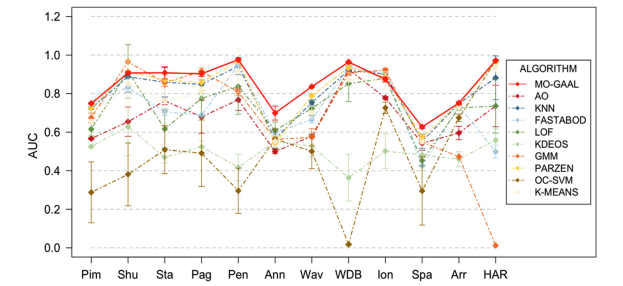
\includegraphics[scale=2]{figures/Result.png}
		\caption{Performance fluctuations of different outlier detectors with different parameters.}
		%The fluctuations are demonstrated by the mean and standard deviation of all experimental results
	\end{figure}
	
	\begin{figure}
		\centering
		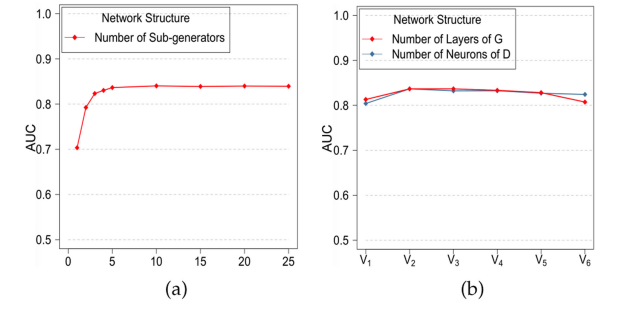
\includegraphics[scale=1.8]{figures/Result 2.png}
		\caption{Experimental results of different network structures on real-world datasets.}
		% Vertical axis represents the average result of a particular network structure on all above real-world datasets
	\end{figure}

  \end{block}

  \begin{block}{CONCLUSIONS}
  	
  	\begin{itemize}
  	\item \textbf{A novel outlier detection algorithm} we proposes a novel outlier detection algorithm SOGAAL, which can directly generate informative potential outliers, to solve the lack of information caused by the curse of dimensionality \\
  	\item \textbf{Strong robustness} MO-GAAL achieves the best average ranking on the real-world datasets, and shows strong robustness to varying parameters.
  	\end{itemize}
  
  \end{block}

\end{column}

\separatorcolumn
\end{columns}
\end{frame}

\end{document}
